%%%%%%%%%%%%%%%%%%%%%%%%%%%%%%%%%%%%%%%%%%%%%%%%%%%%%%%%%%%%%%%%%%%%%%%%%%%%%%%%%%%%%%%%%%
\section{Implementation} \label{sect:implementation}                                     %
%%%%%%%%%%%%%%%%%%%%%%%%%%%%%%%%%%%%%%%%%%%%%%%%%%%%%%%%%%%%%%%%%%%%%%%%%%%%%%%%%%%%%%%%%%

\begin{figure}[ht]
	\centering
	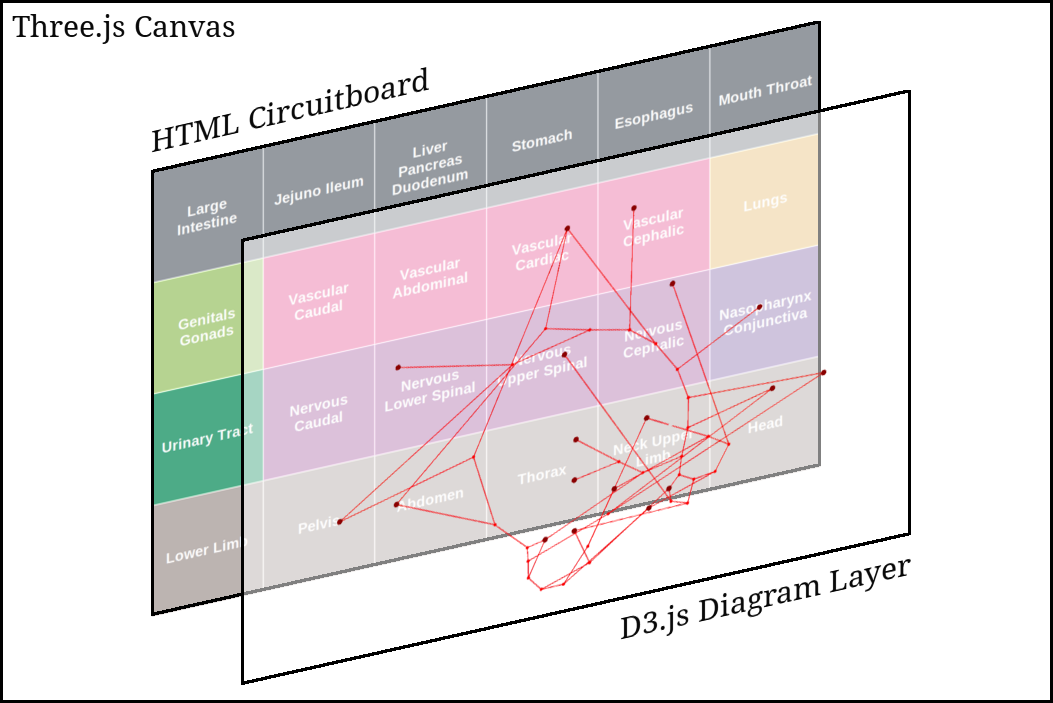
\includegraphics[width=6cm]{images/visual-layers.png}
	\hskip1mm
	\begin{tabular}[b]{lcl}
		\multicolumn{3}{l}{\textbf{Able to Control Position:}}     \\[1mm]
		Three.js Canvas     & $\longrightarrow$ & HTML Treemap     \\[1mm]
		Three.js Canvas     & $\longrightarrow$ & D3.js Layer      \\[3mm]
		
		\multicolumn{3}{l}{\textbf{Able to Add Content:}}          \\[1mm]
		HTML Treemap        & $\longrightarrow$ & D3.js Layer      \\[1mm]
		HTML Treemap        & $\longrightarrow$ & Three.js Canvas  \\[1mm]
		D3.js Layer         & $\longrightarrow$ & Three.js Canvas  \\[10mm]\phantom{x}%hack
	\end{tabular}
	\vskip1mm
	\caption{The three layers of circuitboard visualization and their interaction.}
	\label{fig:visual-layers}
\end{figure}

In this section we discuss a number of implementation aspects of \mbox{ApiNATOMY}.
For maximum compatibility across operating systems as well as handheld devices,
the whole application is written in Javascript. The main framework in use is
AngularJS, which provides a Model-View-Controller architecture, as well as
two-way databinding. Connectivity- and protein-protein
interaction diagrams~(\cref{fig:vascular-connectivity,fig:protein})
are generated using D3.js, and all 3D functionality~(\cref{fig:neurons,fig:protein-3d})
is implemented using Three.js, which provides a convenient abstraction layer over WebGL.



%\subsection{Circuitboard Layers} %%%%%%%%%%%%%%%%%%%%%%%%%%%%%%%%%%%%%%%%%%%%%%%%%%%%%%%%%

The circuit-board is rendered with essentially three layers,
which are shown in \cref{fig:visual-layers}. The treemap is generated
with plain HTML. On top of this, a partly transparent diagram layer is
rendered by D3.js. The positions of the tiles and the positions of the
diagram nodes are synchronized with AngularJS two-way databinding.
When 3D mode is activated, Three.js takes control of both layers.
Besides rendering 3D objects with WebGL, it can manipulate HTML
elements using CSS 3D transforms. When using both rendering engines
in conjunction, Three.js can keep WebGL and HTML perfectly synchronized.
Together with AngularJS two-way databinding, we get very fine control
of positioning. This is demonstrated particularly well in \cref{fig:protein-3d}.
%%
To render \texttt{.swc} neuron files (\cref{fig:neurons}), ApiNATOMY uses SharkViewer,
an open source Three.js library
developed by the Howard Hughes Medical Institute~\cite{weaver_sharkviewer_2014}.

%\subsection{Focus and Direct Feedback} %%%%%%%%%%%%%%%%%%%%%%%%%%%%%%%%%%%%%%%%%%%%%%%%%%%

A separate module keeps track of the entity under focus. Whenever the mouse hovers
over a specific tile or object, it is highlighted and its hierarchical information
is shown in the left side-panel~(\cref{fig:neurons,fig:proteins}). Clicking on the object
fixes this focus, allowing the user to interact with the information in the side-panel.

This direct feedback has another purpose. An ontology need not necessarily be a
tree. In the FMA ontology, for example, different branches may join, making it a
directed acyclic graph. A treemap, however, by its very nature, is only suitable
for visualizing trees. We compensate for this by allowing the same entity to be
represented by more than one tile at the same time. To reinforce this intuition, all
such tiles are highlighted in unison when the mouse hovers over any one of them.
Only one tile per entity is considered `active'. Only the active tile may be opened
up to show its children, and only the active tile participates in the visualization
of cross-tile connectivity data.
